\begin{figure}[ht!]
    \centering
    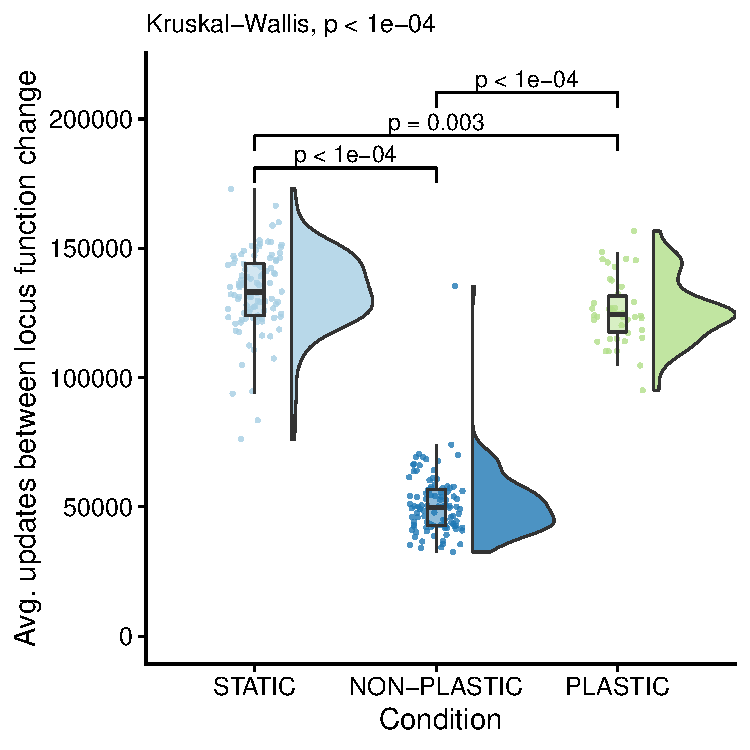
\includegraphics[width=0.33\textwidth]{media/architecture/avg_time_between_func_changes_weighted_mean.pdf}
    \caption{\small
        \textbf{Average time between locus function change.}
        Each replicate of Phase 2A is represented by a single point. 
        Points represent the average time (in updates) between the function of a single locus changing. 
        That is, for a given site in a genome, how many updates pass, on average, before that site is now coding for something else (e.g., the site was coding for the NOT task, but now is not coding for anything). TODO: merge this with another panel of plots? Make a metric out of it?
    }
    \label{fig:architecture_locus_change_time}
\end{figure}